\subsection{Preconditioner: Jacobi}

Look at the $i$-th equation of the system $Au = b, $ $\sum^{N}_{j = 1} a_{ij}u_j = b_i$, this 
can be rewritten in an iterative way

\begin{equation}
\label{eq:jacobi_scaler}
u^{n}_{i} = \frac{1}{a_{ii}}(b_i - \sum_{j \neq i} a_{ij}u^{n-1}_j) \quad \text{which holds for}\quad i = 1,2, ... , N. 
\end{equation}
On the Richardson iteration form this becomes,
\begin{equation}
\label{eq:jacobi_matrix}
u^n = u^{n-1} - D^{-1}(Au^{n-1} - b).
\end{equation}
Here $D^{-1} = (diag(A))^{-1}$ is the preconditioner. The eigenvalues $\mu_k = \cos(\pi k h)$ of the Jacobi matrix 
$J = (I-D^{-1}A)$, are displayed in figure \ref{fig:Jacobi_eigenvalues}. Here $\vert\mu_k\vert$ 
close to $0$ corresponds to high frequent errors and  $\vert\mu_k\vert$ close to $1$ 
corresponds to low frequent error. We recall from the previous section that high frequent error is easily handled, 
while low frequent errors is problematic. Therefor we would like $\vert\mu_k\vert$ close to zero. 


\begin{figure}
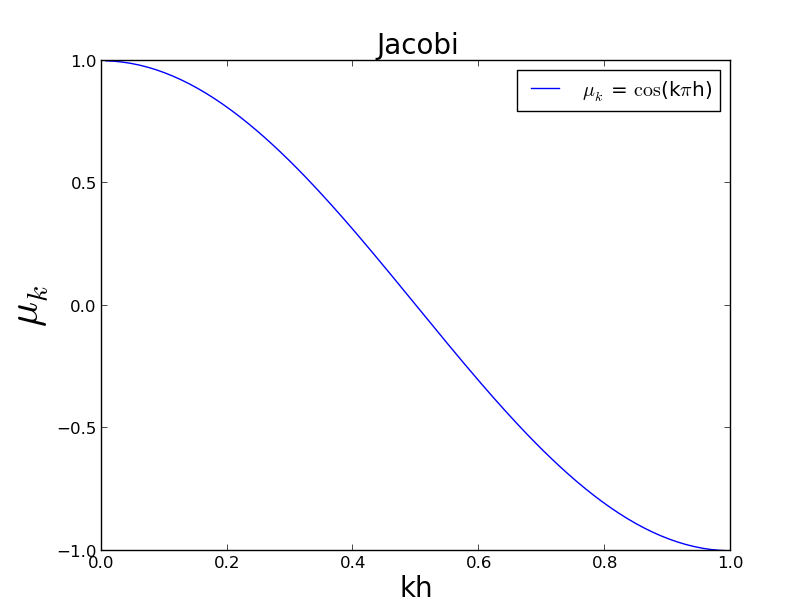
\includegraphics[width=8cm, height=8cm]{chapters/iterative_methods/plots/jacobi_plot}
\caption{Plot of the eigenvalues of the Jacobi method on FDM 
discretized 1D Poisson with $N = 150$ and $\mu_k$ = $\cos(\pi k h )$.}
\label{fig:Jacobi_eigenvalues}
\end{figure}
 

\subsection{Preconditioner: Relaxed Jacobi}
By looking at the Jacobi iteration (\ref{eq:jacobi_scaler}), we see that $u^n_i$ is 
computed based on $u^{n-1}_j$ for $j \neq i$. We can extend (\ref{eq:jacobi_scaler}) by including information 
from the previous iteration $u^{n-1}_i$

\begin{equation}
\label{eq:relaxed_jacobi_scaler}
u^{n}_{i} = (1-\omega)u^{n-1}_i + \frac{\omega}{a_{ii}}(b_i - \sum_{j \neq i} a_{ij}u^{n-1}_j) \quad 
\text{for} \quad i = 1,2, ... , N. 
\end{equation}
On the Richardson iteration form this becomes,
\begin{equation}
\label{eq:jacobi_matrix}
u^n = u^{n-1} - \omega D^{-1}(Au^{n-1} - b).
\end{equation}
The relaxation parameter $\omega$ needs to be chosen. 
By choosing $\omega = 2/3$, we can see from figure \ref{fig:relaxed_Jacobi} that more of  
the eigenvalues correspond to high frequent errors ($\vert \mu_k\vert$ close to $0$). While the 
low frequent error ($\mu_k$ close to $1$) is still a problem. 


\begin{figure}
%\begin{center}
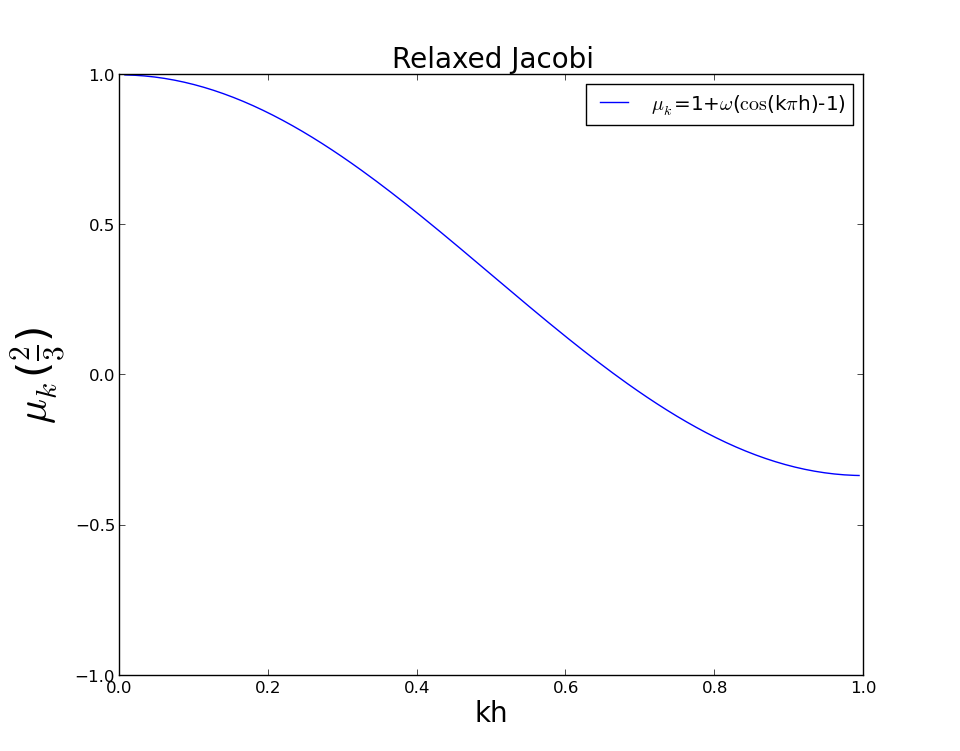
\includegraphics[width=8cm, height=8cm]{chapters/iterative_methods/plots/relax_jacobi_plot}
%\end{center}
\caption{Plot of the eigenvalues of the relaxed Jacobi method on FDM 
discrefized 1D Poisson with $N = 150$ and $\mu_k$ = $1+ \omega(\cos(\pi k h )-1)$.}
\label{fig:relaxed_Jacobi}
\end{figure}

\subsection{Preconditioner: Gauss--Seidel}
A natural extension to the Jacobi iteration (\ref{eq:jacobi_scaler}) is to use $u^n_j$ 
instead of $u^{n-1}_j$ for $j < i$ in the sum, since these values is already computed. 
This method is known as the Gauss--Seidel iteration, 
 
\begin{equation}
\label{eq:GS_scaler}
u^{n}_{i} = \frac{1}{a_{ii}}(b_i - \sum_{j < i} a_{ij}u^{n}_j - \sum_{j > i} a_{ij}u^{n-1}_j) 
\quad \text{for}\quad i = 1,2, ... , N. 
\end{equation}
Let $A = D + U + L$, where D is the diagonal, U is the upper diagonal part and L is 
the lower diagonal part of A. On the Richardson iteration form this becomes,
\begin{equation}
\label{eq:GS_matrix}
u^n = u^{n-1} - (D + L)^{-1}(Au^{n-1} - b).
\end{equation}
We can apply the same ideas for the relaxed Jacobi and get a relaxed Gauss--Seidel,
\begin{equation}
\label{eq:GS_scaler}
u^{n}_{i} = (1-\omega)u^{n-1}_i  + \frac{\omega}{a_{ii}}(b_i - \sum_{j < i} a_{ij}u^{n}_j - \sum_{j > i} a_{ij}u^{n-1}_j) 
\quad \text{for}\quad i = 1,2, ... , N. 
\end{equation}
On the Richardson iteration form,
\begin{equation}
\label{eq:GS_matrix} 
u^n = u^{n-1} - \omega(D + L)^{-1}(Au^{n-1} - b).
\end{equation}
Note that Gauss--Seidel is not symmetric (unless A is a diagonal matrix). As mention above, 
these methods handles high frequent error well, while the low frequent errors remains almost unchanged.
The low frequent errors can be handled by multigrid methods. 


